\chapter{Preliminaries}


\section{Notations}
In the following sections, we will express the points in the Euclidean plane in lowercase letters. For example, when we defined terminal points in section 1.3, we used lowercase letters $q$ and $p$. Also, we  may need  the notations for segments, rays and lines in definitions, theorems or proofs. Here are some rules for them. A segment $\overline{ab}$ is a straight line segment from the point $a$ to the point $b$. A ray from $a$ to $b$ is denoted as $\overrightarrow{ab}$. And a line $ab$ means a line passing though $a$ and $b$. An angle donation $\angle aob$ means an angle from ray $\overrightarrow{oa}$ to  ray $\overrightarrow{ob}$ in the counterclockwise direction. 






\section{Chains}
\begin{definition}
We define a finite sequence of distinct disks $\mathcal{O} = (O_1, O_2, \dots, O_n)$ be a \textbf{chain} if
\begin{enumerate}
    \item for $1\le i \le n-1$, every two consecutive disk $O_i$ ad $O_{i+1}$ intersect but do not contain each other. Then, for every disks $O_i$, define the \textbf{connecting arcs} of $O_i$ as the arcs on the boundary of $O_i$ in $O_{i-1}$  and in $O_{i+1}$, and denote as $C_{i}^{i-1}$ and $C_{i}^{i+1}$ respectively;
    \item The connecting arcs $C_{i}^{i-1}$ and $C_{i}^{i+1}$ for $2\le i\le n-1$ can share an endpoint but they do not overlap.
\end{enumerate}
\end{definition}


\begin{figure}[ht]
\centering
\begin{subfigure}{.8\textwidth}
\centering
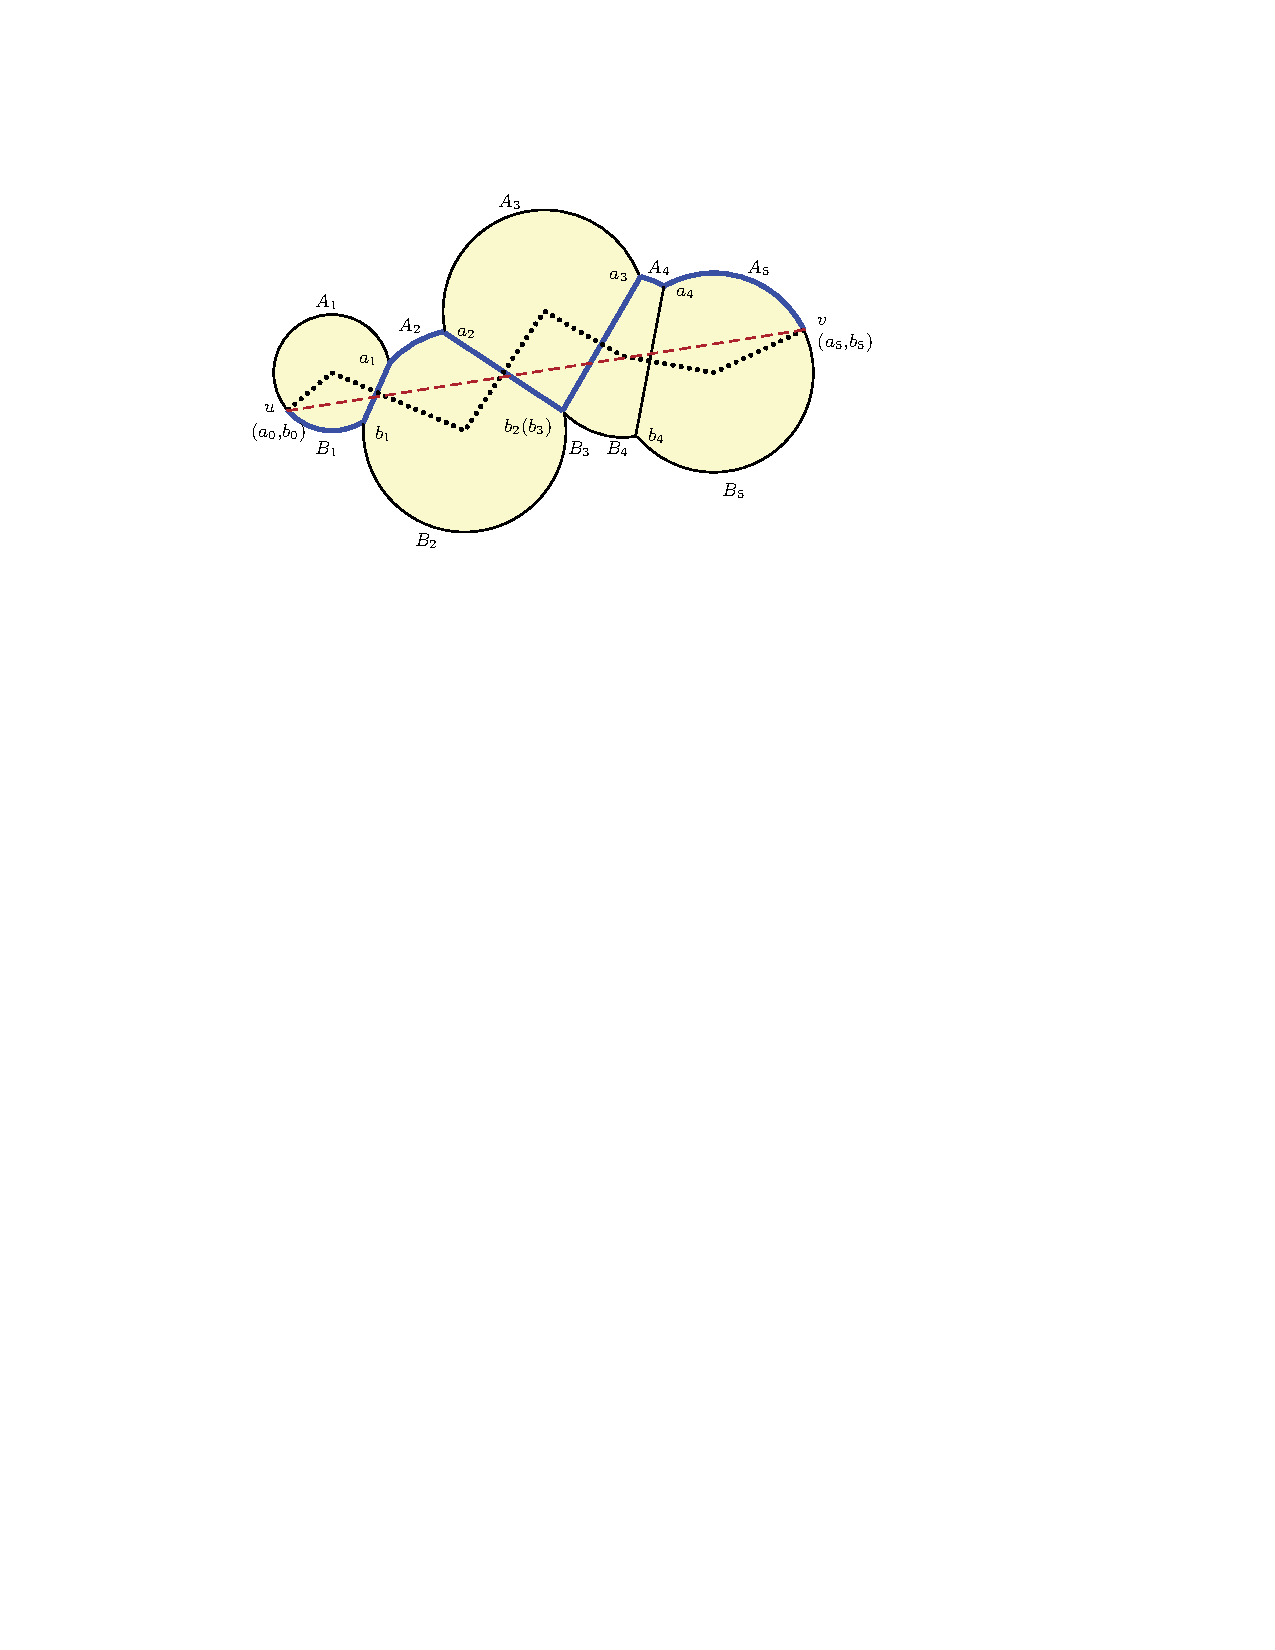
\includegraphics[width=.9\linewidth]{Figures/xia_a.pdf}
\caption{} \label{fig:xia_a}
\end{subfigure}
% \hspace*{\fill}

\begin{subfigure}{.8\textwidth}
\centering
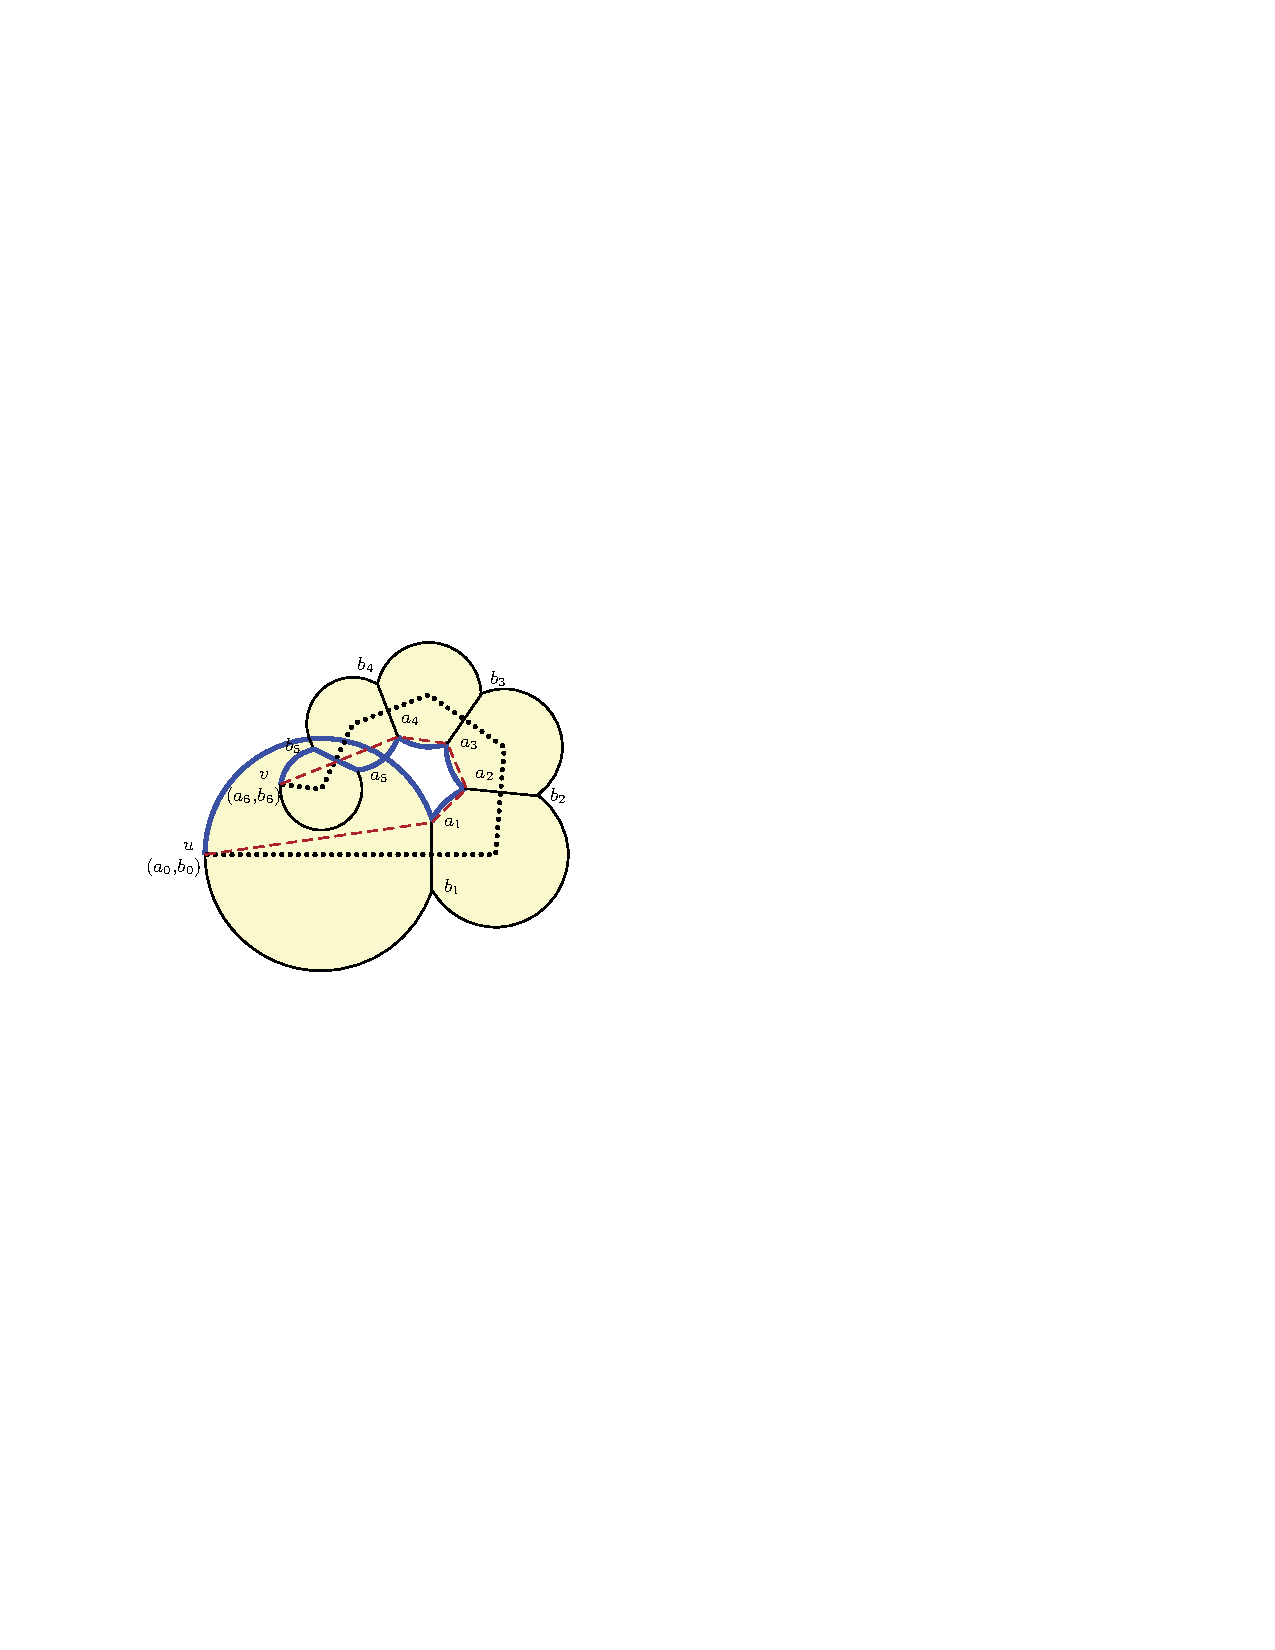
\includegraphics[width=.6\linewidth]{Figures/xia_b.pdf}
\caption{} \label{fig:xia_b}
\end{subfigure}
% \hspace*{\fill} % separation between the subfigures
\caption[Two illustrations of chains]{Two illustrations of chains. Terminal points $u$ and $v$ are unobstructed in Figure~\ref{fig:xia_a}. And Figure~\ref{fig:xia_b} shows the obstructed case.  Reprinted from \cite{xia}.} \label{fig:xia}
\end{figure}



\begin{definition}
Given a  chain $\mathcal{O} = \{O_1, O_2, \dots, O_n\}$. Choose points $u$ and $v$ on the boundary of $O_1$ and $O_n$  respectively. We say $u$ and $v$ are a pair of \textbf{terminal points} of $\mathcal{O}$. Denote the centers of $O_1, O_2, \dots, O_n$ as {$\boldsymbol{o_1, o_2, \dots, o_n}$} respectively. Then,  the \textbf{center polyline} between $u$ and $v$ is the polyline $uo_1\dots o_nv$. For $1\le i\le n-1$, let $\boldsymbol{a_i}$ and $\boldsymbol{b_i}$ be the intersections of the boundaries of $O_i$ and $O_{i+1}$. Without loss of generality, we say $a_i$'s are all on one side of the centered polyline, and $b_i$'s are on the other side. Also, define $\boldsymbol{a_0}=\boldsymbol{b_0} = u$ and $\boldsymbol{a_n}=\boldsymbol{b_n} = v$. For each disk $O_i$, denote the two arcs between the straight line segments $\overline{a_ib_i}$ and $\overline{a_{i-1}b_{i-1}}$ on the boundary of $O_i$ as $\boldsymbol{A_i}$ and $\boldsymbol{B_i}$, where $A_i$ has two end points $a_{i-1}$ and $a_i$ and $B_i$ has $b_{i-1}$ and $b_i$.
\end{definition}


\begin{definition}
Define $\boldsymbol{D_{\mathcal{O}}(u, v)}=up_1\dots p_{n-1}v$  as the shortest polyline from $u$ to $v$ that consists of line segments $\overline{up1}, \overline{p1p2}$, \dots, $\overline{p_{n-1}v}$ where $p_i\in\overline{a_ib_i}$ for $1\le i\le n-1$. That is, $D_{\mathcal{O}}(u, v)$
is the shortest polyline from $u$ to $v$ that intersects line segments $\overline{a_1b_1},\dots,\overline{a_{n-1}b_{n-1}}$ in order. Also, $\boldsymbol{|D_{\mathcal{O}}(u, v)|}$, the length of $D_{\mathcal{O}}(u, v)$, is the sum of lengths of all line segments in $D_{\mathcal{O}}(u, v)$.  
We say $u$ and $v$ are \textbf{obstructed} if the polyline $D_{\mathcal{O}}(u, v)$ contains a point $p_j$ which is either $a_j$ or $b_j$ for some $1\le j\le n-1$.
\end{definition}


\begin{proposition}
If $u$ and $v$ are not unobstructed, $ D_{\mathcal{O}}(u, v)$ is a straight line. 
\end{proposition}

\section{From Chains to Arcgons}
\begin{proposition}
Chains with unobstructed terminal points are equivalent to arcgons. 
\end{proposition}

\begin{proof}
We prove  the proposition by first expressing chains in graphs and then showing the expression in graph is equivalent to arcgons.

Let $\mathcal{O} = \{O_1, O_2, \dots, O_n\}$ be an  arbitrary chain. Suppose our terminal points $u$ and  $v$ are obstructed. Then, construct a graph $G$ whose edges are $\{A_1, A_2, \dots, A_n\}\cup \{B_1, B_2, \dots, B_n\} \cup \{\overline{a_1b_1},\overline{a_2b_2}, \dots \overline{a_{n-1}b_{n-1}} \}$, and vertices are $\{a_0, a_1, a_2, \dots, a_n\}\cup \{b_0, b_1, b_2, \dots, b_n\}$. Then, for all $1\le i\le n$, let $f_i$ be a graph constructed with $A_i, B_i, \overline{a_{i-1}a_i}$ and $\overline{b_{i-1}b_i}$. It is clear that $f_i$ is a face with a base circle $O_i$, and $F=\{f_1, f_2, \dots, f_n\}$ is a valid arcgon. Therefore, chains with unobstructed terminal points are equivalent to arcgons. 

On the other hand, suppose an arcgon $F=\{f_1, f_2, \dots, f_n\}$ is given. Let $\mathcal{C} = \{C_1, C_2, \dots, C_n\}$ be the base circles of $F$. Consider the disk bounded by each circle. Denote them as $\{O_1, O_2, \dots, O_n\}.$ Then, we can show that $\mathcal{O} = \{O_1, O_2, \dots, O_n\}$ is a chain with unobstructed terminal points. We know very two consecutive disks intersect because every consecutive faces share a diagonal in $F$. Also, since the arcgon $F$ is planar graph, the neighboring disks of every disk do not overlap. Therefore, all arcgons are chains with unobstructed terminal points.

We have shown the proposition.
\end{proof}


% \section{More on Arcgons}





% [Arcgon with condition 6 == chain with unobstructed terminal points]




% \begin{enumerate}
%     \item arcgon: modify there or explain more here about the p, q. The p, q is the same as p, q in chains. That is, any points on two end arcs are valid. but not for critical arcgons with complexity. of 1 b/c for paths over and below and one passing at least one diagonal, they must have the equal length. Thus, critical arcgons means fixed p and q.
    
%     \item define complexity.
    
%     Every stretch factor at most 
% \end{enumerate}


% arcgon